% Homework template for Inference and Information
% UPDATE: September 26, 2017 by Xiangxiang
\documentclass[a4paper]{article}
\usepackage{ctex}
\usepackage{amsmath, amssymb, amsthm}
\usepackage{moreenum}
\usepackage{mathtools}
\usepackage{url}
\usepackage{bm}
\usepackage{enumitem}
\usepackage{graphicx}
\usepackage{listings}
\usepackage{color}

\lstset{
    basicstyle          =   \sffamily,          % 基本代码风格
    keywordstyle        =   \bfseries,          % 关键字风格
    commentstyle        =   \rmfamily\itshape,  % 注释的风格,斜体
    stringstyle         =   \ttfamily,  % 字符串风格
    flexiblecolumns,                % 别问为什么,加上这个
    numbers             =   left,   % 行号的位置在左边
    showspaces          =   false,  % 是否显示空格,显示了有点乱,所以不现实了
    numberstyle         =   \zihao{-5}\ttfamily,    % 行号的样式,小五号,tt等宽字体
    showstringspaces    =   false,
    captionpos          =   t,      % 这段代码的名字所呈现的位置,t指的是top上面
    frame               =   lrtb,   % 显示边框
}

\lstdefinestyle{Python}{
    language        =   Python, % 语言选Python
    basicstyle      =   \zihao{-5}\ttfamily,
    numberstyle     =   \zihao{-5}\ttfamily,
    keywordstyle    =   \color{blue},
    keywordstyle    =   [2] \color{teal},
    stringstyle     =   \color{magenta},
    commentstyle    =   \color{red}\ttfamily,
    breaklines      =   true,   % 自动换行,建议不要写太长的行
    columns         =   fixed,  % 如果不加这一句,字间距就不固定,很丑,必须加
    basewidth       =   0.5em,
}
\usepackage{subcaption}
\usepackage{booktabs} % toprule
\usepackage[mathcal]{eucal}
\usepackage[thehwcnt = 5]{iidef}

\thecourseinstitute{清华大学电子工程系}
\thecoursename{\textbf{媒体与认知} \space 课堂2}
\theterm{2021-2022学年春季学期}
\hwname{作业}
\begin{document}
\courseheader{}
\name{李智毅}
\vspace{3mm}
\centerline{\textbf{\Large{理论部分}}}

\section{单选题(15分)}
\subsection{\underline{B}}

\subsection{\underline{D}}

\subsection{\underline{B}}

\subsection{\underline{D}}

\subsection{\underline{C}}

\section{计算题(15 分)}
% 计算题1
\subsection{隐含马尔可夫模型的解码}

\hspace{2em}某手机专卖店今年元旦新开业,每月上旬进货时,由专卖店经理决策,采用三种进货方案中的一种:高档手机(H),中档手机(M),低档手机(L)。

\hspace{2em}当月市场行情假设分为畅销($S_1$)和滞销($S_2$)两种。畅销时,三种进货方案的概率分别为0.4, 0.4, 0.2;滞销时,三种进货方案的概率分别为0.2, 0.3, 0.5。

\hspace{2em}某月份市场行情为畅销,下一个月份为畅销和滞销的概率分别为0.6 和0.4;某月份市场行情为滞销,下一个月份为畅销和滞销的概率分别为0.5 和0.5。

\hspace{2em}开业第一个月市场行情为畅销和滞销的可能性均为0.5。

\vspace{3mm}
(1) 如果我们采用隐含马尔可夫模型(HMM)对该专卖店进货环节建模,{\color{blue}请写出HMM对应的参数$\lambda=\{\pi, A, B\}$}。

$$ \mathbf{\pi} = \left[ 0.5, 0.5 \right] $$
$$ \mathbf{A} = \left[ \begin{array}{cc}
    0.6 & 0.4 \\
    0.5 & 0.5
\end{array} \right] $$
$$ \mathbf{B} = \left[ \begin{array}{ccc}
    0.4 & 0.4 & 0.2 \\
    0.2 & 0.3 & 0.5
\end{array} \right] $$

\vspace{3mm}
(2) 在第一季度中,采购业务员执行的进货方案为“高档手机,中档手机,低档手机”,即观测序列为H, M, L。{\color{blue}请利用Viterbi算法推测前三个月的市场行情}。
$$ \delta_1(1) = \pi_1 b_1(H) = 0.2 $$
$$ \delta_1(2) = \pi_2 b_2(H) = 0.1 $$
$$ \varphi_1(1) = 0 $$
$$ \varphi_1(2) = 0 $$
$$ \delta_2(1) = \max{\left\{\delta_1(1) P(S_1 | S_1), \delta_1(2) P(S_1 | S_2)\right\}} b_1(M) = 0.048 $$
$$ \delta_2(2) = \max{\left\{\delta_1(1) P(S_2 | S_1), \delta_1(2) P(S_2 | S_2)\right\}} b_2(M) = 0.024 $$
$$ \varphi_2(1) = S_1 $$
$$ \varphi_2(2) = S_1 $$
$$ \delta_3(1) = \max{\left\{\delta_2(1) P(S_1 | S_1), \delta_2(2) P(S_1 | S_2)\right\}} b_1(L) = 0.00576 $$
$$ \delta_3(2) = \max{\left\{\delta_2(1) P(S_2 | S_1), \delta_2(2) P(S_2 | S_2)\right\}} b_2(L) = 0.0096 $$
$$ \varphi_2(1) = S_1 $$
$$ \varphi_2(2) = S_1 $$
因此,可以推知最优状态序列为$ S_1, S_1, S_2 $ \\
即市场行情为:畅销、畅销、滞销。

% 计算题2
\subsection{循环神经网络的长时相关性建模能力}

\hspace{2em}对序列中的长距离相关信息进行建模是涉及序列的任务中十分重要的一点,例如在阅读理解任务里,题目和正文中的关键词可能相距很远,这就需要模型具备足够好的长距离相关信息建模能力。传统RNN在训练时存在梯度消失问题,较远的误差无法得到有效传递,因此学习长距离相关信息时面临较大挑战,在本题中我们对传统RNN难以学习长距离相关信息的问题进行一个简单的讨论。

\hspace{2em}对RNN的计算过程进行简化,考虑一个暂不采用激活函数以及输入x的RNN:
\begin{equation*}
    \bm{h}_t = U\bm{h}_{t-1} = U \left( U\bm{h}_{t-2} \right) = ... = U^t\bm{h}_0
\end{equation*}
\hspace{2em}其中$U^t$为$t$个$U$矩阵连乘。若矩阵$U$存在如下特征值分解:
\begin{equation*}
    U = Q \Lambda Q^\top
\end{equation*}
\hspace{2em}其中$Q$为单位正交矩阵(每一列为模长为1的特征向量),$Q^\top$为$Q$的转置,Λ为特征值对角矩阵,则上述的RNN计算过程可表示为:
\begin{equation*}
    \bm{h}_t = Q \Lambda^t Q^\top \bm{h}_0
\end{equation*}

\vspace{3mm}
本题目包含以下三个问题:

(1) 假设某一特征值$\lambda_i < 1$,{\color{blue}当时刻$t$增大时,$\Lambda^t$中第$i$行$i$列的值会怎样变化?}\\
由
$$ \left( \mathbf{\Lambda}^t \right)_{ii} = \lambda_i^t $$
因此,当$ \lambda_i^t < 1 $时,对应元素$ \left( \mathbf{\Lambda}^t \right)_{ii} $应会趋于$ 0 $.\\

(2) 假设$\bm{h}_0=\bm{q}_i$,其中$\bm{q}_i$为$U$矩阵的第$i$个特征向量(即Q的第$i$列),设$\mathcal{L}$为目标函数计算出的loss。{\color{blue}试验证:
\begin{equation*}
    \frac{\partial \mathcal{L}}{\partial \bm{h}_0} = \lambda_i^t \frac{\partial \mathcal{L}}{\partial \bm{h}_t}
\end{equation*}}
由于$ \bm{h}_0=\bm{q}_i $,因此
$$ \bm{h}_t = U^t \bm{h}_0 = U^t \bm{q}_i = \lambda_i^t \bm{q}_i $$
其中$ \lambda_i $为$ U $的第$ i $个特征向量。因此,有
$$ \frac{\partial \bm{h}_t}{\partial \bm{h}_0} = \lambda^t $$
$$ \frac{\partial \mathcal{L}}{\partial \bm{h}_0} = \frac{\partial \mathcal{L}}{\partial \bm{h}_t} \frac{\partial \bm{h}_t}{\partial \bm{h}_0} = \lambda_i^t \frac{\partial \mathcal{L}}{\partial \bm{h}_t} $$

(3) 对于更一般的$\bm{h}_0$,由于$Q$中的特征向量构成一组完备正交基,可以将$\bm{h}_0$分解为$Q$中不同特征向量的线性组合,即$\bm{h}_0=\sum_{i=1}^{n}k_i\bm{q}_i$。通过上述分析,{\color{blue}请尝试解释传统RNN训练中的梯度消失现象},由此理解传统RNN对长距离相关信息建模的困难。\\
根据$ \bm{h}_0 = \sum_{i=1}^{n} k_i \bm{q}_i $,因此有
$$ \frac{\partial \mathcal{L}}{\partial \bm{h}_0} = \sum_{i=1}^{n} k_i \frac{\partial \mathcal{L}}{\partial \bm{q}_i} = \sum_{i=1}^n k_i \lambda_i^t \frac{\partial \mathcal{L}}{\partial \bm{h}_t} $$
因此,可以看出,在做长距离相关信息建模的过程中,$ t $较大,因此在$ \lambda_i $均小于$ 1 $时会出现梯度消失现象,导致建模困难。\\

% 请根据是否选择自选课题的情况选择“编程作业报告”或“自选课题开题报告”中的一项完成
\section{编程作业报告}
\subsection{完成基于循环神经网络的场景文本识别程序代码}
按照要求完成网络的搭建,以及训练、测试代码,运行“network.py”验证网络输出维度,结果(如图1所示)\\
\begin{figure}
    \centering
    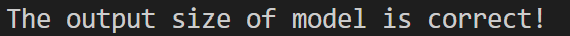
\includegraphics[width=8cm]{Fig_1.png}
    \caption{测试网络输出维度}
\end{figure}

\subsection{模型的训练和验证}
运行 "python main.py --mode train",使用默认参数训练模型,得到以下数据(图2):\\
训练轮数(epoch):40 \\
验证集准确率:50.0\% \\
\begin{figure}
    \centering
    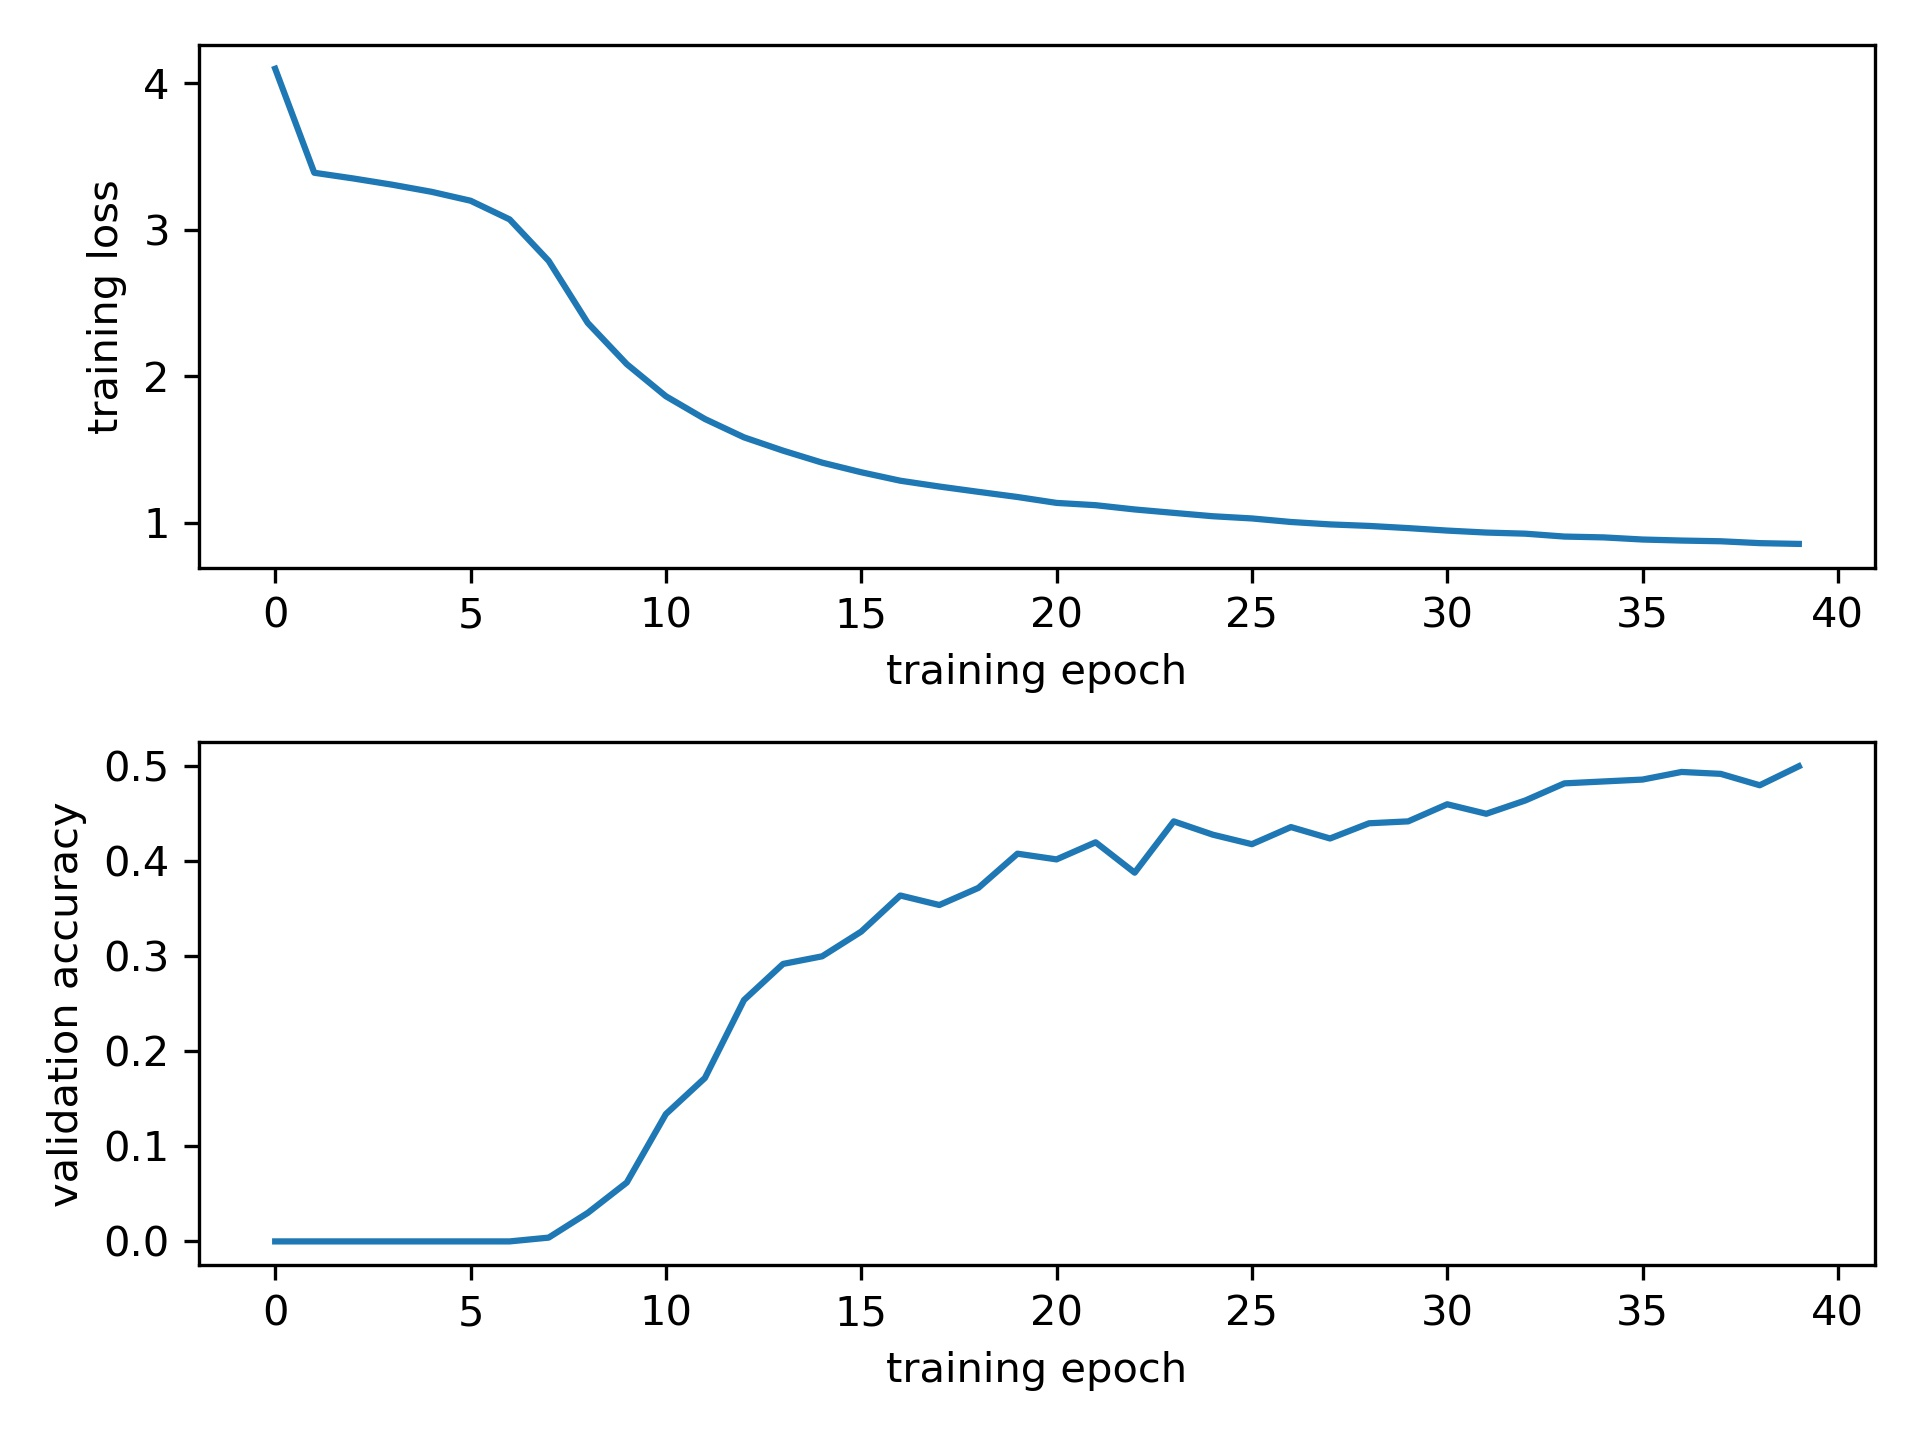
\includegraphics[width=12cm]{Fig_2.jpg}
    \caption{默认参数训练曲线}
\end{figure}

\subsection{使用训练好的模型预测新的文本图像}
使用训练好的模型"model\_epoch40.pth"预测文本图像(图3),有结果(图4) \\
\begin{figure}
    \centering
    
\includegraphics[width=12cm]{Fig_3.png}
    \caption{待预测文本图像}
\end{figure}
\begin{figure}
    \centering
    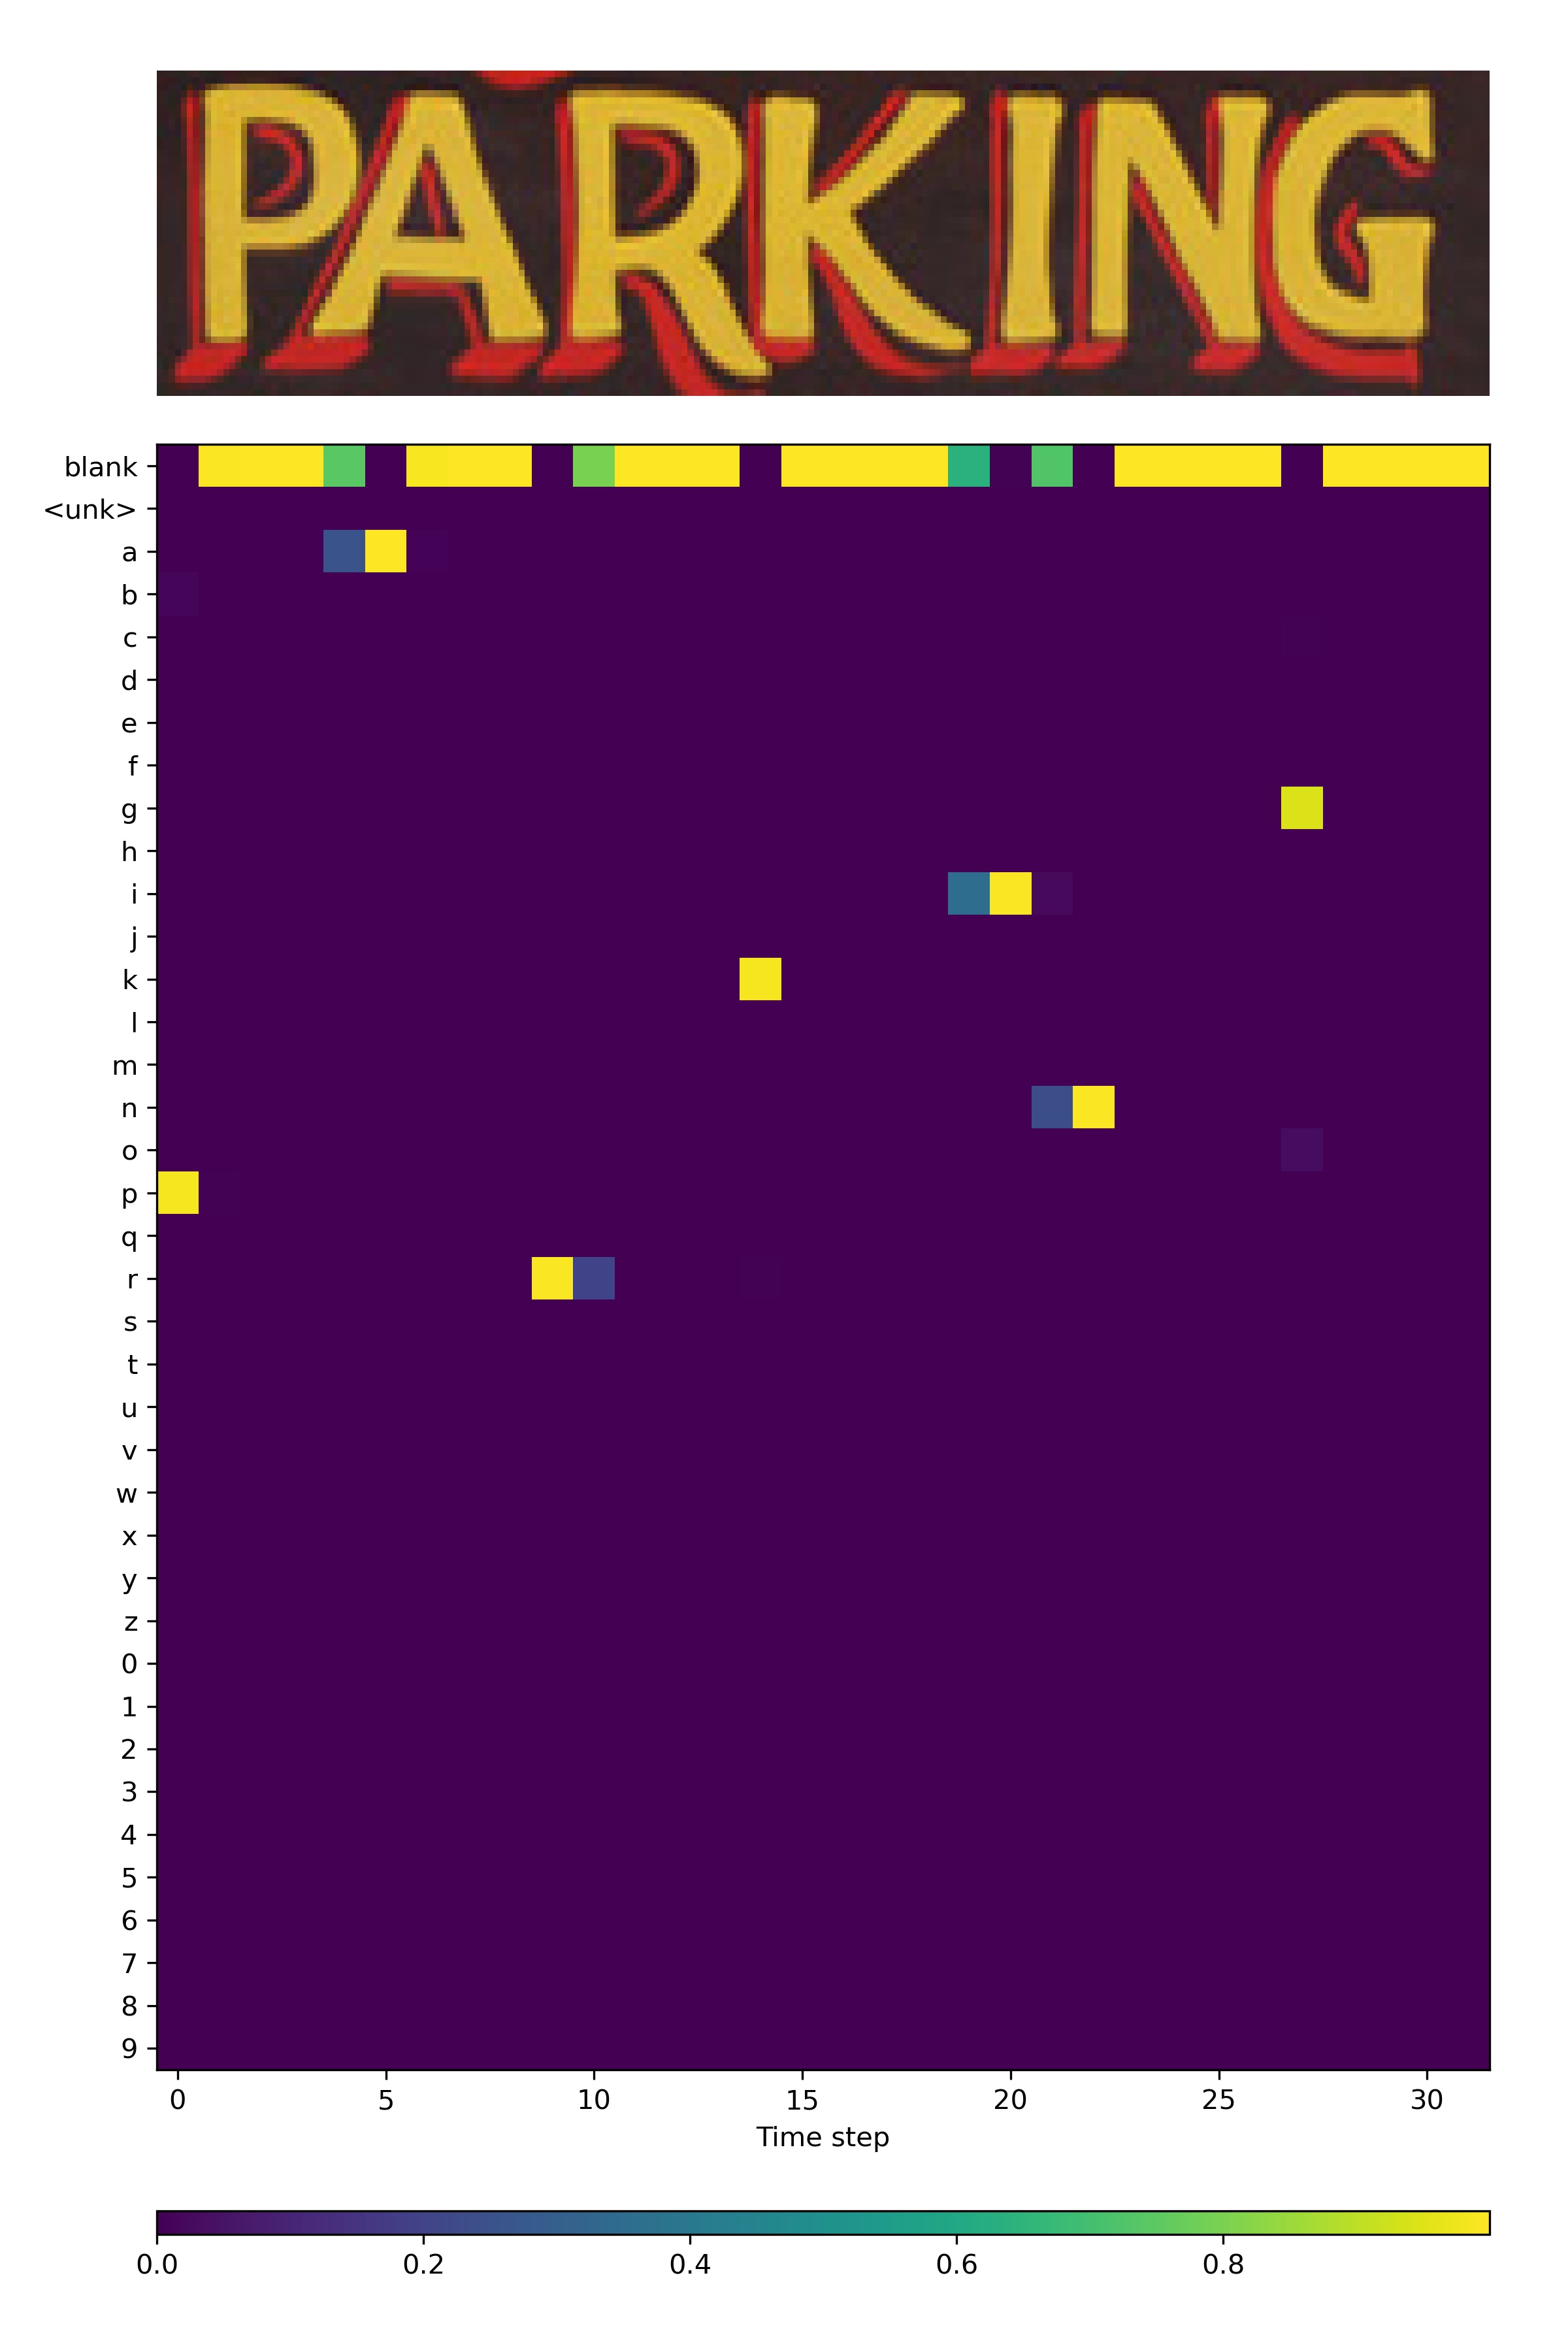
\includegraphics[width=12cm]{Fig_4.jpg}
    \caption{40轮训练模型预测结果}
\end{figure}
预测结果:parking\\
从预测结果可以看出,对图像的识别结果为每一个正确字符后接上若干空白字符,使用CTC算法可以得到正确的预测结果。\\
以下分别使用训练10轮模型(图5)、训练20轮模型(图6)、训练30轮模型(图7)对图像(图3)进行预测,有如图所示结果。\\
训练10轮模型预测(图5):parrin \\
可以看出,此时模型能够具有一定的识别能力,但对于每个字符的估计准确性都不高,模型有待进一步训练 \\
\begin{figure}
    \centering
    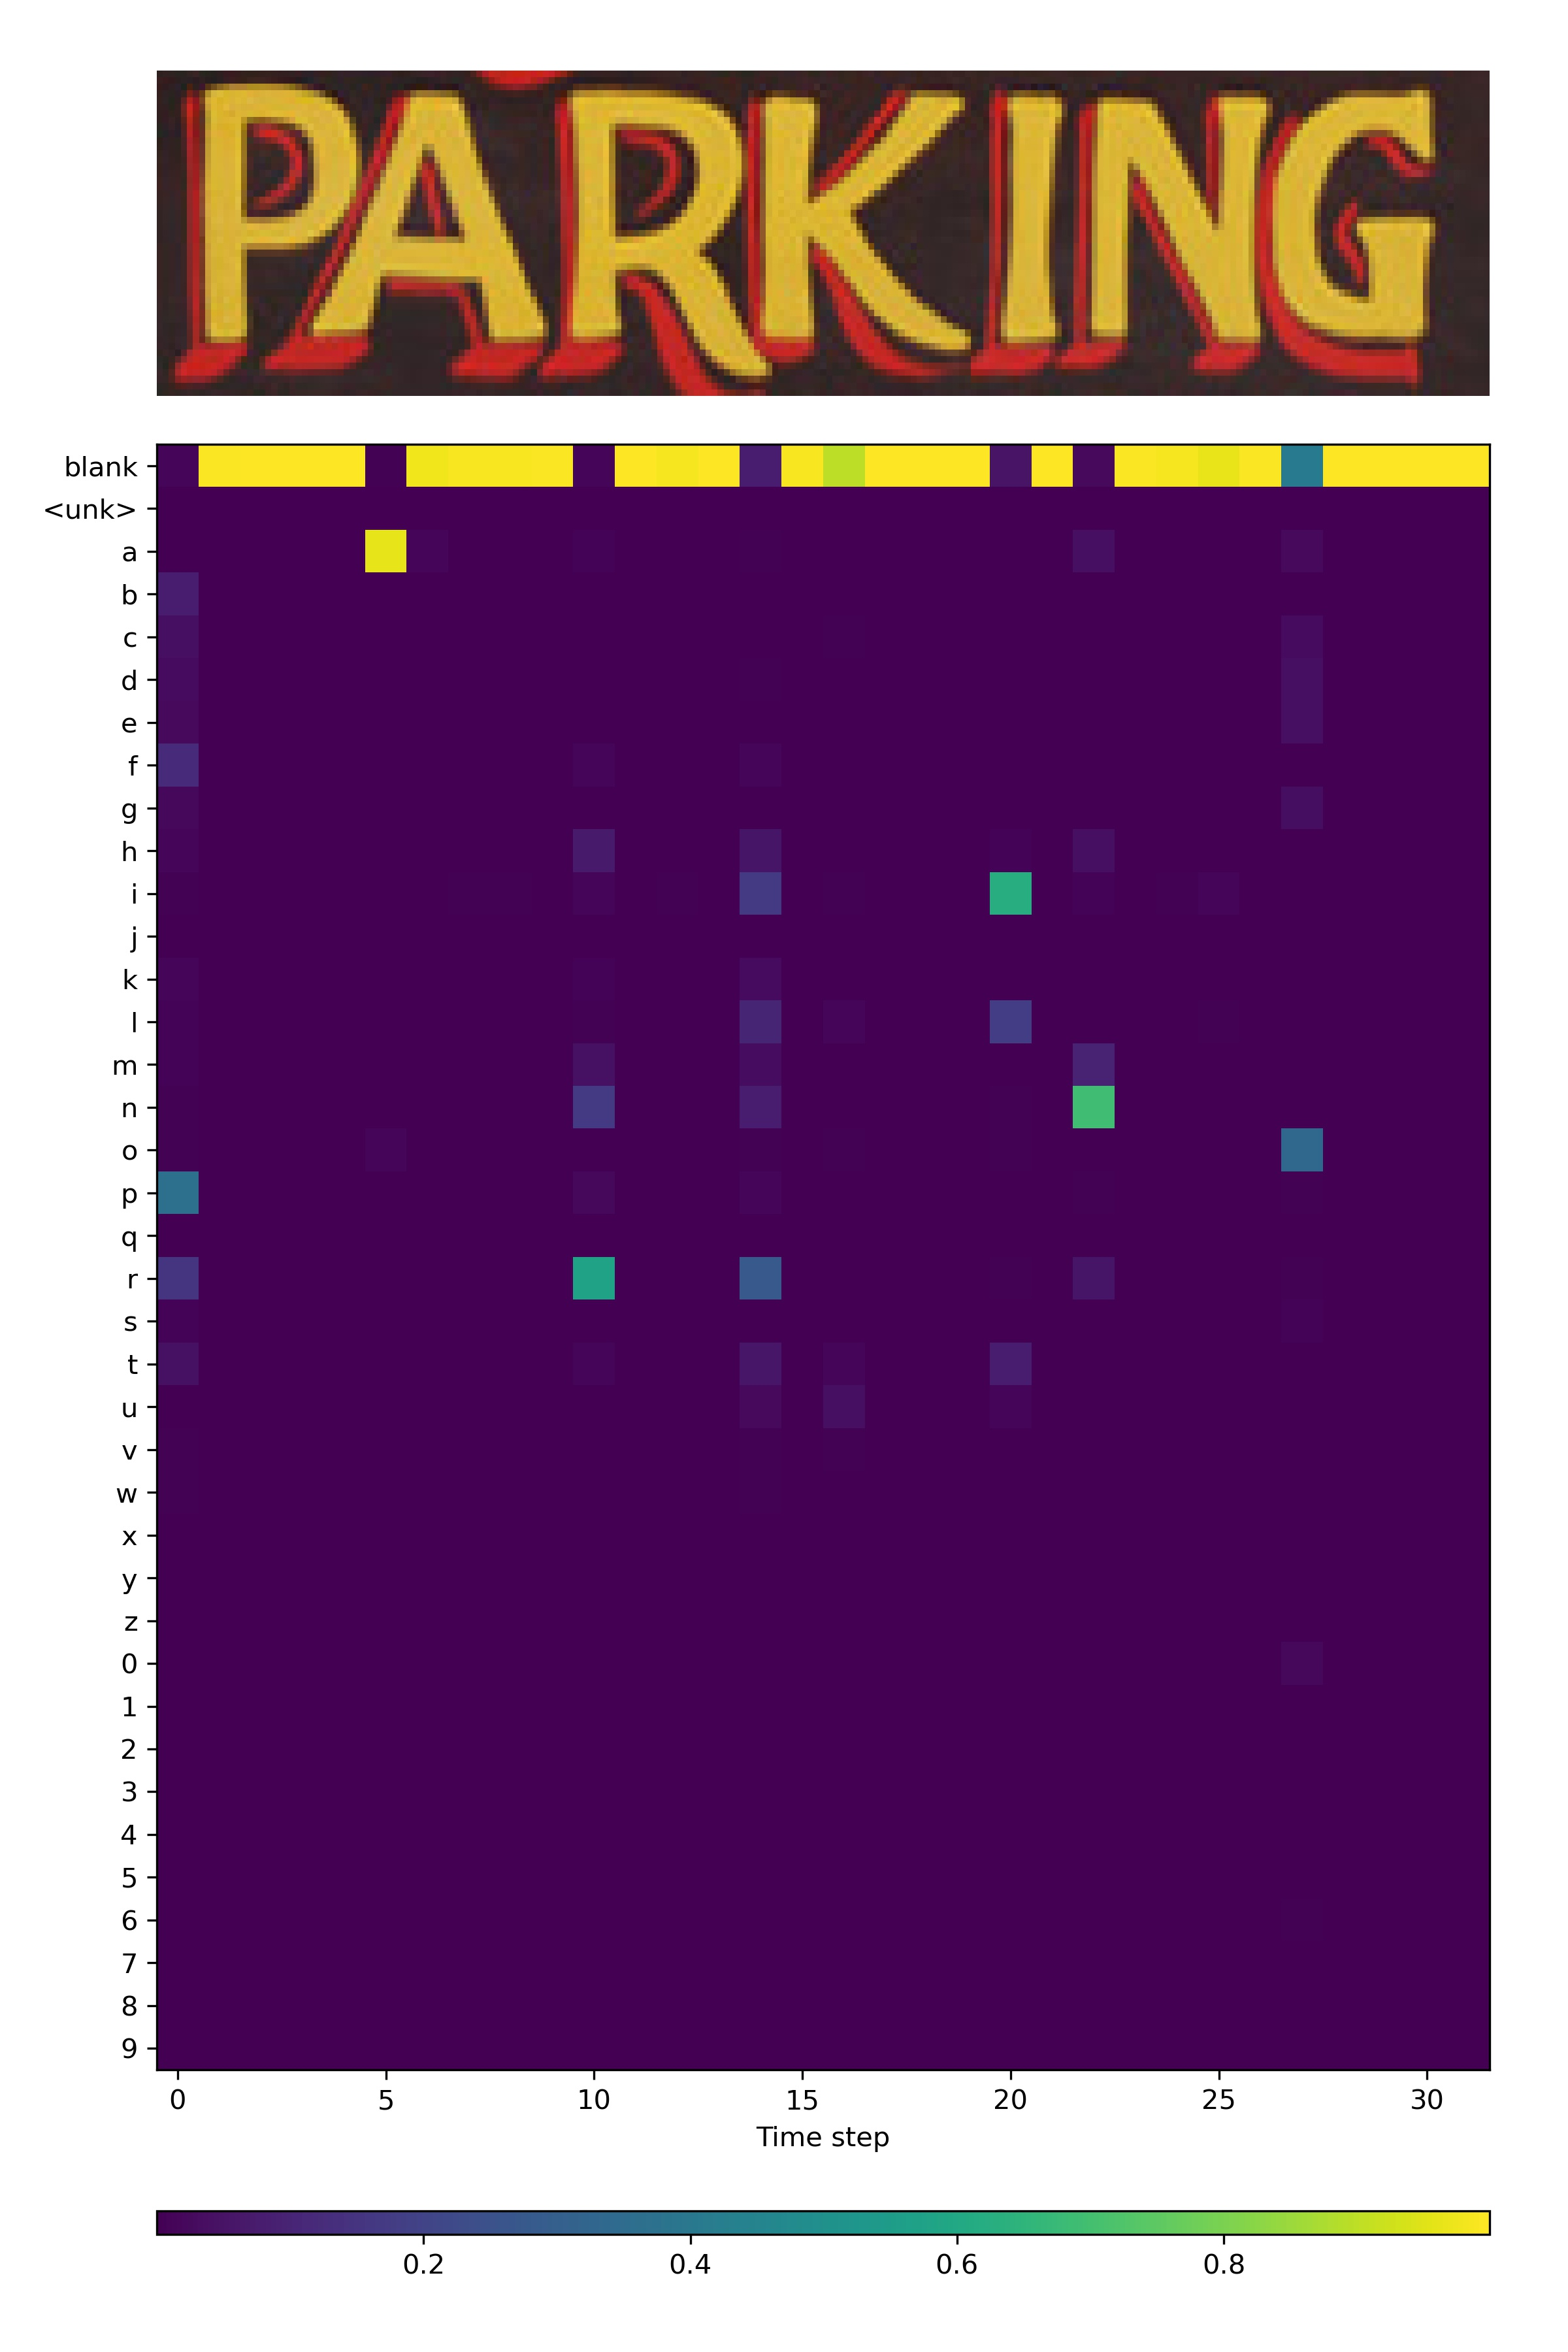
\includegraphics[width=12cm]{Fig_5.jpg}
    \caption{10轮训练模型预测结果}
\end{figure}
训练20轮模型预测(图6):parking \\
\begin{figure}
    \centering
    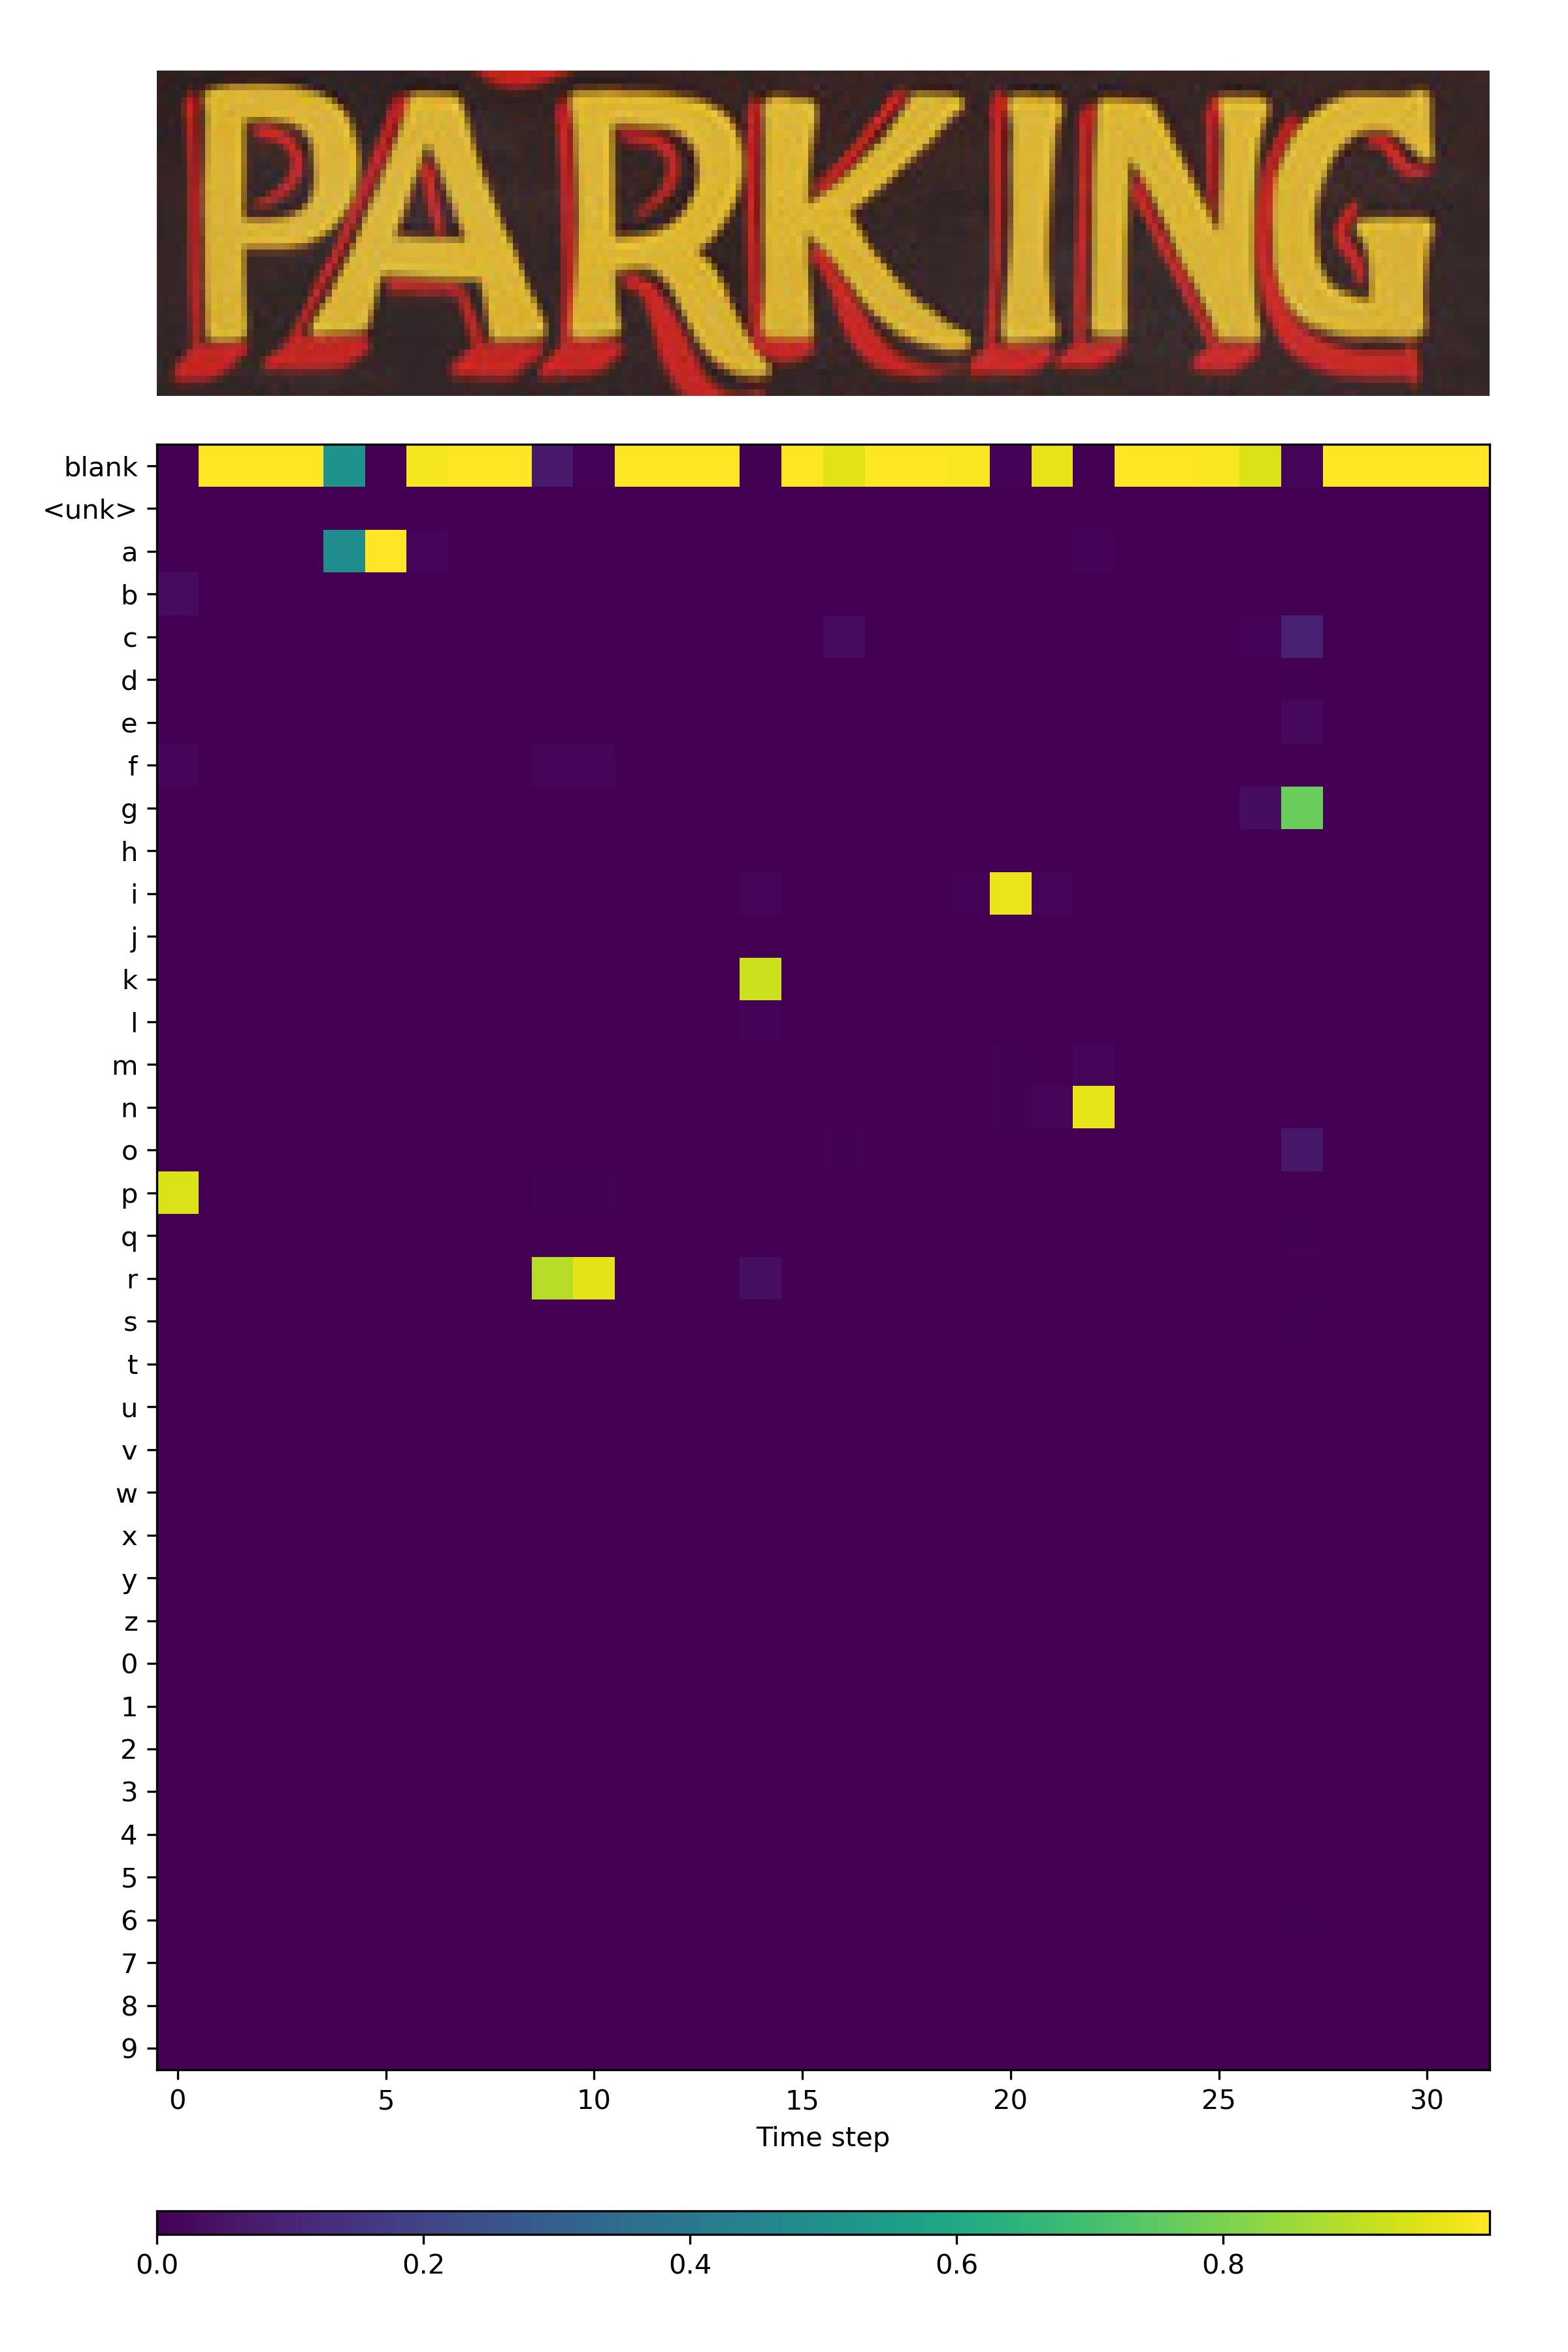
\includegraphics[width=12cm]{Fig_6.jpg}
    \caption{20轮训练模型预测结果}
\end{figure}
训练30轮模型预测(图7):parking \\
\begin{figure}
    \centering
    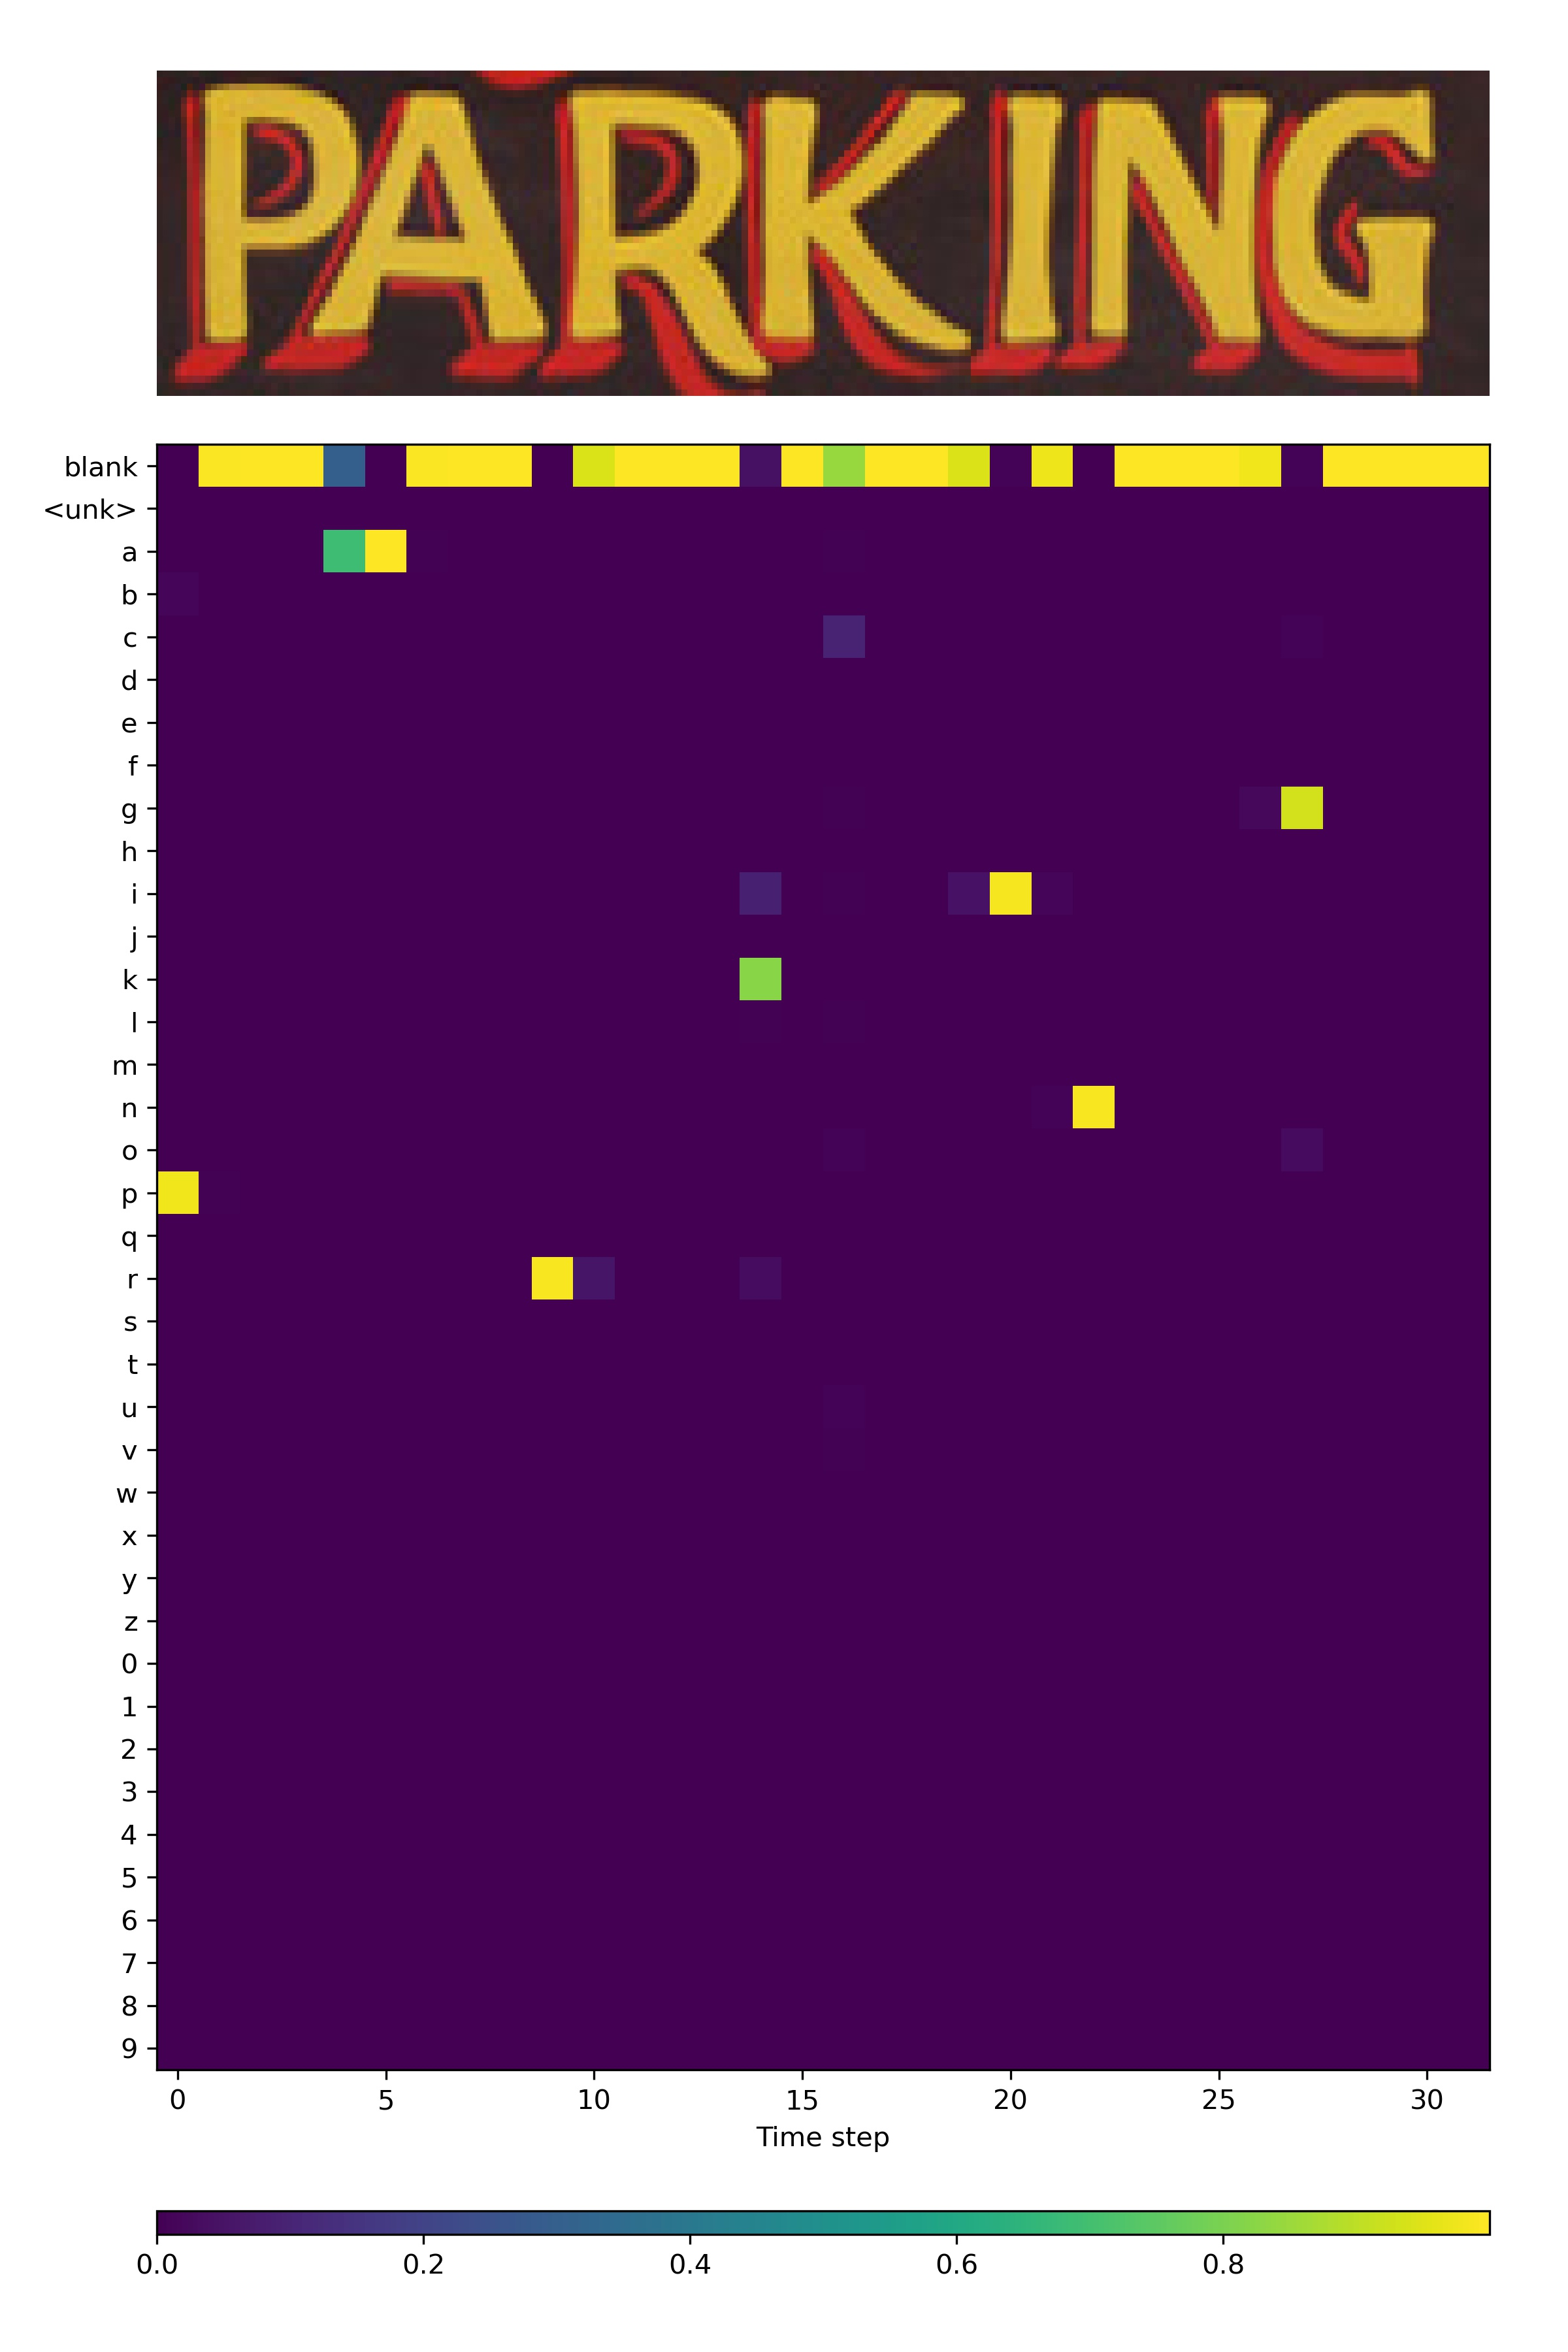
\includegraphics[width=12cm]{Fig_7.jpg}
    \caption{30轮训练模型预测结果}
\end{figure}
可以看出,在第20轮后,对该图像的预测就较为准确了。\\

\end{document}



%%% Local Variables:
%%% mode: late\rvx
%%% TeX-master: t
%%% End:
